\subsection{Database}
	All'interno dell'architettura sono utilizzati:
	\begin{itemize}
		\item un database relazionale, PostgreSql, che viene usato per il salvataggio delle configurazioni dei gateway, delle informazioni di utenti ed enti, oltre alle impostazioni dei grafici creati dagli utenti stessi;
		\item un database non relazionale, Timescale, che viene usato per salvare i dati inviati dai dispositivi, le logs degli eventi e gli alert con i valori anomali rilevati. 
	\end{itemize}
	Entrambi i database sono rilasciati tramite dockerfile, tramite il quale ne viene effettuata una prima configurazione.
	\subsubsection{Timescale}
	La struttura del database non relazionale è la seguente:
	\begin{itemize}
		\item Sensors
		\begin{itemize}
			\item time: timestamptz
			\item real\_sensor\_id: integer
			\item real\_device\_id: integer
			\item gateway\_name: text
			\item value: double
		\end{itemize}
		\item Alerts
		\begin{itemize}
			\item time: timestamptz
			\item real\_sensor\_id: integer
			\item real\_device\_id: integer
			\item gateway\_name: text
			\item value: double
		\end{itemize}
		\item Logs
		\begin{itemize}
			\item time: timestamptz
			\item user\_id: integer
			\item ip\_address: varchar
			\item operation: text
			\item data: text
		\end{itemize}
	\end{itemize}
	\subsubsection{PostgreSql}
	La struttura del database SQL è rappresentata nello schema logico sottostante:
		
			\begin{landscape}
			\begin{figure}[H]
				\centering
				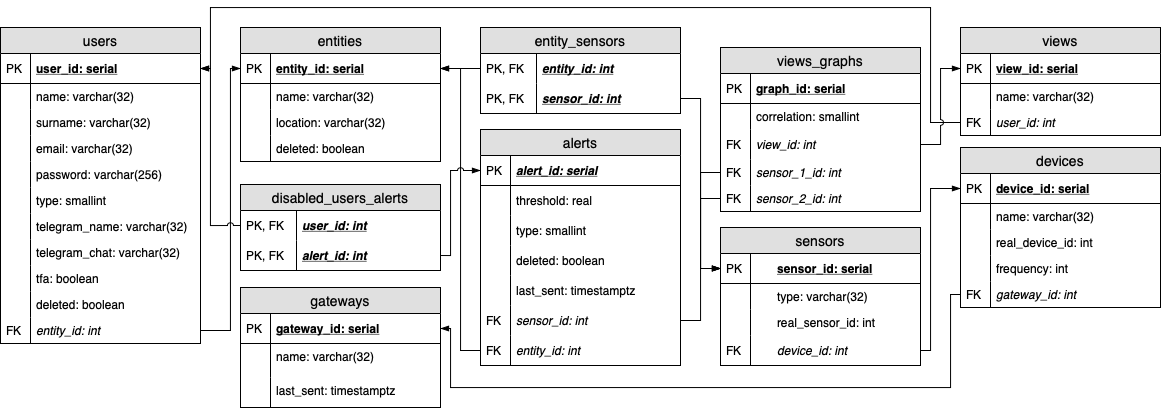
\includegraphics[scale=0.600]{res/images/DATABASE/ER_Modificato.png}
				\caption{Diagramma logico del database relazionale}
				\label{Diagramma 9}
			\end{figure}
			\end{landscape}		
	 